\section{引言}\label{ux5f15ux8a00}

\section*{Introduction}

早期眼底筛查是眼科疾病诊断的有效方法，能够反映视网膜、视盘、血管和黄斑区域的多类病变征象。通过对眼底图像进行分析，有助于患者发现潜在病变并尽早干预，从而降低不可逆的视力损伤甚至视力丧失的风险。随着眼底筛查规模扩大，人工阅片面临阅片耗时、依赖专家经验和基层医疗资源不足等问题，因此基于眼底图像的眼科疾病诊断具有重要应用价值\hyperref[_Ref213949315]{{[}1{]}}。围绕眼底筛查，现有方法大体可分为传统机器学习、视觉语言模型和卷积神经网络三类路线。传统机器学习通常依赖图像增强、病灶分割、纹理或形态等人工特征，再结合支持向量机、随机森林等分类器完成识别\hyperref[_RefRahman2022MLFundus]{{[}2{]}}，这类方法具有一定可解释性，但特征设计依赖先验经验，对复杂眼底病灶和多疾病共存场景的表达能力有限。近年来，视觉大语言模型为眼底图像理解、图文联合分析和医学报告生成提供了新的研究方向\hyperref[_RefLim2024VLVOphthalmology]{{[}3{]}}\hyperref[_RefUrooj2025LLMMedicalImage]{{[}4{]}}，但其训练和微调通常依赖大规模高质量标注数据、图文配对数据以及较高算力资源，在医疗数据稀缺、隐私受限和临床部署资源有限的场景中仍面临较高成本。相比之下，以CNN为代表的深度视觉模型能够直接从眼底图像中学习局部纹理、病灶区域和空间结构特征，已广泛应用于疾病识别\hyperref[_Ref213871637]{{[}5{]}}、病灶分割\hyperref[_Ref213948625]{{[}6{]}}、医学图像重建\hyperref[_Ref213948898]{{[}7{]}}和疾病诊断与预测\hyperref[_Ref213949262]{{[}8{]}}等任务。因此，本文选择CNN作为多标签眼科疾病识别任务的基础路线。然而，在真实临床部署中，基于CNN的眼科疾病识别方法仍面临多疾病共存、跨机构部署泛化性能下降以及隐私保护等挑战。具体而言：

Early fundus screening is an effective approach for ocular disease diagnosis, as it can reveal diverse pathological signs in the retina, optic disc, blood vessels, and macular region. Analyzing fundus images helps identify potential lesions and supports early intervention, thereby reducing the risk of irreversible visual impairment or even vision loss. As fundus screening continues to expand, manual fundus screening is limited by its time cost, dependence on expert experience, and shortage of primary medical resources. Fundus-image-based ocular disease diagnosis therefore has important practical value\hyperref[_Ref213949315]{{[}1{]}}. Existing methods for fundus screening can be broadly grouped into three technical directions: ML, VLM, and CNN. ML methods usually rely on hand-crafted features such as image enhancement, lesion segmentation, texture, or morphology, followed by classifiers such as support vector machines or random forests for recognition\hyperref[_RefRahman2022MLFundus]{{[}2{]}}. These methods offer a degree of interpretability, but their feature design depends heavily on prior experience and has limited capacity to represent complex fundus lesions and multi-disease co-occurrence. In recent years, VLM has opened new directions for fundus image understanding, image-text joint analysis, and medical report generation\hyperref[_RefLim2024VLVOphthalmology]{{[}3{]}}\hyperref[_RefUrooj2025LLMMedicalImage]{{[}4{]}}. However, their training and fine-tuning generally require large-scale high-quality annotations, paired image-text data, and substantial computational resources, which remain costly when medical data are scarce, privacy is restricted, and clinical deployment resources are limited. In contrast, CNN-based deep visual models can directly learn local textures, lesion regions, and spatial structural features from fundus images, and have been widely applied to disease recognition\hyperref[_Ref213871637]{{[}5{]}}, lesion segmentation\hyperref[_Ref213948625]{{[}6{]}}, medical image reconstruction\hyperref[_Ref213948898]{{[}7{]}}, and diagnosis and prediction of ocular diseases\hyperref[_Ref213949262]{{[}8{]}}. Therefore, we adopt CNN as the main modeling backbone for multi-label ocular disease recognition. Nevertheless, in real-world clinical deployment, CNN-based ocular disease recognition methods still face challenges including multi-disease co-occurrence, degraded generalization performance across institutions, and privacy preservation. Specifically:

1.在临床眼科疾病诊断中，单只眼睛可能同时存在多种疾病，若仍采用标准单标签分类器或将不同疾病完全独立建模，容易造成误检与漏检\hyperref[_Ref213949362]{{[}9{]}}。近年来，自然图像中也存在多标签识别方法的相关工作，比如ML-GCN \hyperref[_Ref213949382]{{[}10{]}}，通过统计各标签出现的频率建立图关联性，使得识别出某个标签后，更有可能识别出其关联标签，从而减少漏检。而在多标签眼科疾病识别中，各疾病之间的关联性更加错综复杂，仅靠标签频率来建立疾病关联性的方法对于这种复杂情况效果可能不可靠。因此，面向眼底图像的多疾病共存场景，仍需要探索一种更高效可靠的标签-特征关联性构建方法。

1. In clinical ocular disease diagnosis, a single eye may present multiple diseases simultaneously. Using a standard single-label classifier, or modeling different diseases as fully independent, can therefore lead to false positives and false negatives\hyperref[_Ref213949362]{{[}9{]}}. Multi-label recognition has also been widely studied for natural images. For example, ML-GCN\hyperref[_Ref213949382]{{[}10{]}} constructs graph relevance from label occurrence frequencies, making relevant labels more likely to be recognized once a given label is identified and thereby reducing false negatives. However, in multi-label ocular disease recognition, disease relevance is more complex, and methods that infer disease relevance solely from label frequencies may be unreliable. For multi-disease co-occurrence in fundus images, a more reliable method for label-feature relevance construction is therefore needed.

2.医疗图像数据与自然图像不同，其标注通常需要专业医生完成，数据获取和标注成本较高；同时，不同医疗机构之间还存在数据共享限制、标签空间不统一等问题，使多源域数据的访问与协同训练并不总是容易实现。然而，即使通过某个医疗机构的训练集训练得到了一个性能良好的模型，将其应用到另外的机构时，目标域数据也常因成像设备、光照条件和人工处理流程差异产生域偏移\hyperref[_Ref213949348]{{[}11{]}}，导致模型性能下滑。如\figsubref{fig:intro-domain-gap}{a1}和\figsubref{fig:intro-domain-gap}{a3}所示，源域和目标域的分布有差异，仅在源域训练的base model（\figsubref{fig:intro-domain-gap}{b1}）得到的决策边界可能不适用于目标域分布（\figsubref{fig:intro-domain-gap}{b2}）。常见的域适应方法DA选择将源域和目标域数据一同送入模型训练来对齐域分布\hyperref[_Ref213949354]{{[}12{]}}，但这需要训练阶段访问目标域数据；多源域泛化方法虽可避免访问目标域，但通常依赖多个源域共同训练。在医疗数据协同训练受限的实际场景中，上述前提往往难以满足。因此，探索仅利用单一源域提取域不变特征的单域泛化方法，更符合跨机构部署需求。

2. Medical images differ from natural images because their annotations usually require professional physicians, making both data acquisition and annotation costly. In addition, data sharing restrictions and inconsistent label spaces across medical institutions often limit access to multi-source-domain data and collaborative training. Even when a model performs well on the training set of one medical institution, applying it to another institution can introduce domain shift in the target domain because of differences in imaging devices, illumination conditions, and manual processing procedures\hyperref[_Ref213949348]{{[}11{]}}, resulting in performance degradation. As shown in \hyperref[fig:intro-domain-gap]{Fig.~\ref*{fig:intro-domain-gap}.a1} and \hyperref[fig:intro-domain-gap]{Fig.~\ref*{fig:intro-domain-gap}.a3}, the distributions of the source domain and target domain differ. The decision boundary learned by a base model trained only on the source domain (\hyperref[fig:intro-domain-gap]{Fig.~\ref*{fig:intro-domain-gap}.b1}) may not fit the target-domain distribution (\hyperref[fig:intro-domain-gap]{Fig.~\ref*{fig:intro-domain-gap}.b2}). Common domain adaptation (DA) methods align domain distributions by jointly using source-domain and target-domain data during model training\hyperref[_Ref213949354]{{[}12{]}}, but this requires access to target-domain data during training. Although multi-source domain generalization methods avoid access to the target domain, they usually rely on joint training across multiple source domains. In practical settings where collaborative training with medical data is restricted, these assumptions are often hard to meet. Therefore, exploring single domain generalization methods that extract domain-invariant features using only a single source domain better matches the needs of cross-institutional deployment.

\begin{figure}[H]
\centering
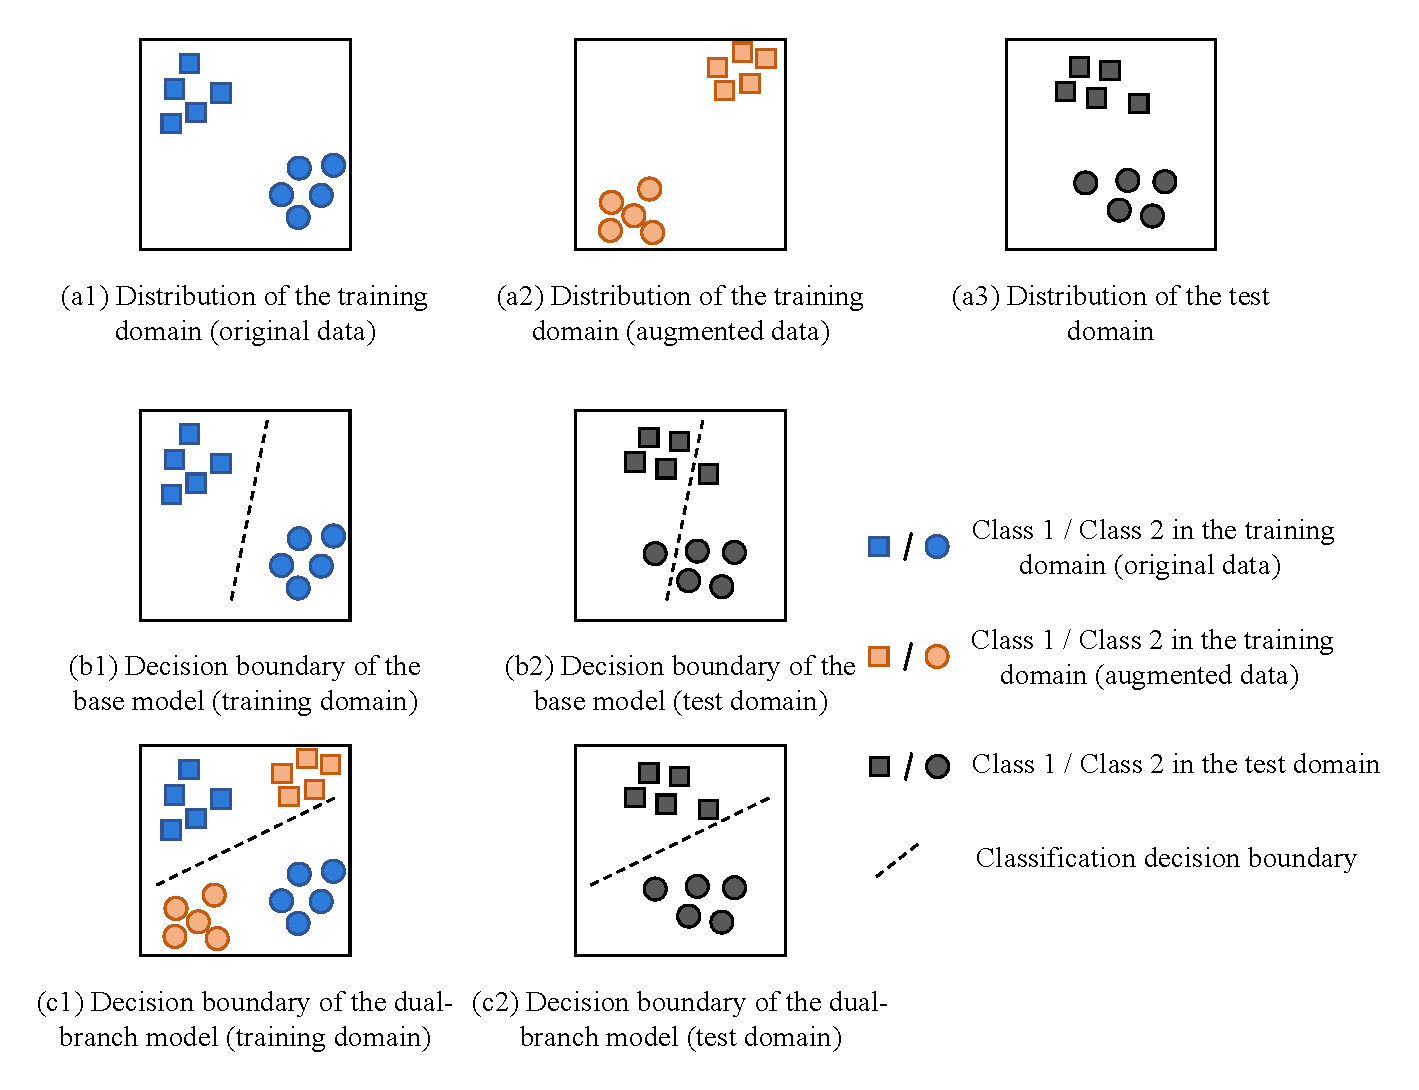
\includegraphics[width=0.72\textwidth]{./images/media/image1_padded.pdf}
\caption{域偏移场景下常规模型与双分支模型决策边界示意图。(a) 展示源域原始图像（训练集）、源域增强图像和目标域（测试集）的数据分布关系，其中源域增强图像用于模拟目标域可能出现的分布差异；(b) 仅利用源域原始图像训练时，模型学习到的决策边界可能不适用于目标域，因而在目标域样本上产生分类错误；(c) 利用源域原始图像与源域增强图像构建双分支结构，并结合对比学习与 CAM 引导，提取域不变特征后，模型能够学习到更适用于未知域的决策边界。 Schematic illustration of the decision boundaries of a conventional model and a dual-branch model under domain shift. (a) shows the distribution relationship among original source-domain images (training set), augmented source-domain images, and the target domain (test set), where augmented source-domain images are used to simulate possible distribution shifts in the target domain. (b) When the model is trained only with original source-domain images, the learned decision boundary may not fit the target domain and can therefore cause classification errors on target-domain samples. (c) By constructing a dual-branch structure with original and augmented source-domain images and incorporating contrastive learning with CAM guidance, the model extracts domain-invariant features and learns a decision boundary that is more applicable to unseen domains.}
\label{fig:intro-domain-gap}
\end{figure}

3.医疗数据比起自然图像更加敏感，存在更高的隐私泄露风险。常见的攻击方法可以通过模型的训练梯度逆向恢复出患者的数据\hyperref[_Ref213949393]{{[}13{]}}。针对此问题，目前已有联邦学习、同态加密、安全多方计算和差分隐私等隐私保护方法研究，但是隐私保护与模型性能之间通常存在trade-off关系；尤其在DA场景中，源域和目标域数据需要同时参与训练，可能带来隐私机制添加复杂、多域性能衰减明显等问题。因此，需要在单域泛化训练流程中进一步探索隐私保护与模型性能之间的平衡方法。

3. Medical data are more sensitive than natural images and therefore involve higher privacy leakage risk. Common attack methods can recover patient data from model training gradients\hyperref[_Ref213949393]{{[}13{]}}. To address this issue, privacy-preserving methods such as federated learning, homomorphic encryption, secure multi-party computation, and differential privacy have been investigated. However, privacy preservation usually comes with a privacy-performance trade-off. In DA scenarios in particular, source-domain and target-domain data must participate in training simultaneously, which can complicate the integration of privacy mechanisms and cause more severe performance degradation across domains. It is therefore necessary to further explore how to balance privacy preservation and model performance within the single domain generalization training process.

为应对上述三个关键挑战，我们构建了一个面向多标签眼科疾病识别的可解释与隐私保护单域泛化框架。针对眼科疾病识别中普遍存在的多疾病共存问题，我们引入基于 Transformer 的自适应标签-特征关联性构建模块，通过自注意力机制建模标签关联，并利用交叉注意力机制将标签语义与对应的图像特征进行融合，在标签层面与特征层面同时构建疾病共现依赖，从而减少多标签识别中的误检与漏检；针对多机构数据访问受限与跨机构部署域偏移并存的问题，我们提出双分支引导域不变特征提取模块，仅利用单一源域数据进行训练，通过对源域原始图像及其风格扰动后的源域增强图像构建双分支结构（如\figsubref{fig:intro-domain-gap}{a1}和\figsubref{fig:intro-domain-gap}{a2}所示），在特征层面挖掘两者的共性表示。同时，引入 CAM（Class Activation Mapping） 作为先验引导，促使模型聚焦于疾病相关区域，从而抑制域特定噪声的学习，使得模型能够形成更适用于未知域分布的决策边界（\figsubref{fig:intro-domain-gap}{c1}），并在未知域上保持稳定的识别性能（\figsubref{fig:intro-domain-gap}{c2}）。此外，CAM 还能够可视化模型关注区域，增强模型的可解释性；针对跨域医疗场景下的隐私泄露风险，本文在单域泛化训练过程中集成自适应高斯差分隐私机制，通过在梯度更新阶段注入噪声实现隐私保护。在中等隐私预算下，该机制能够在不显著牺牲模型性能的前提下提供有效的隐私保护，实现跨域泛化能力与隐私保护的兼顾。

To address the above three key challenges, we build a privacy-preserving interpretable single domain generalization framework for multi-label ocular disease recognition. For the common issue of multi-disease co-occurrence in ocular disease recognition, we introduce a Transformer-based Adaptive Label-Feature Relevance Construction (ARC) module. It models label relevance using Transformer self-attention and fuses label semantics with corresponding image features using Transformer cross-attention, thereby constructing disease co-occurrence dependencies at both the label and feature levels to reduce false positives and false negatives in multi-label recognition. To handle restricted multi-institutional data access together with cross-institutional domain shift, we propose a Dual-Branch Guided Domain-Invariant Feature Extraction (DFE) module. This module is trained using only a single source domain and constructs a dual-branch structure from original source-domain images and style-disturbed augmented source-domain images, as shown in \hyperref[fig:intro-domain-gap]{Fig.~\ref*{fig:intro-domain-gap}.a1} and \hyperref[fig:intro-domain-gap]{Fig.~\ref*{fig:intro-domain-gap}.a2}, to learn their shared representations at the feature level. Meanwhile, Class Activation Mapping (CAM) is introduced as prior guidance to encourage the model to focus on disease-related regions and suppress the learning of domain-specific noise. This enables the model to form a decision boundary that is more suitable for unseen-domain distributions (\hyperref[fig:intro-domain-gap]{Fig.~\ref*{fig:intro-domain-gap}.c1}) and to maintain stable recognition performance on unseen domains (\hyperref[fig:intro-domain-gap]{Fig.~\ref*{fig:intro-domain-gap}.c2}). In addition, CAM visualizes model-attended regions and enhances model interpretability. To address privacy leakage risk in cross-domain medical scenarios, we integrate an Adaptive Gaussian Differential Privacy (AdaGDP) mechanism into the single domain generalization training process and provide privacy preservation by injecting noise during gradient updates. Under a moderate privacy budget, this mechanism preserves privacy without substantially sacrificing model performance, thereby jointly supporting cross-domain generalization and privacy preservation.

最后，在多个具有代表性的眼底图像数据集上进行的泛化实验表明，该框架在保持良好可解释性的同时，提升了跨域多标签识别性能，并在隐私保护场景下表现稳定。

Finally, generalization experiments on several representative fundus image datasets show that the framework improves cross-domain multi-label recognition performance while maintaining good interpretability, and it remains stable under privacy-preserving scenarios.

我们的贡献如下：

The main contributions of this study are summarized as follows:

\begin{sloppypar}
1.提出了一种自适应标签-特征关联性构建模块（Adaptive label-feature relevance construction, ARC），基于 Transformer 的自注意力机制与交叉注意力机制，在标签层面与特征层面同时建模疾病共现依赖，有效降低了多标签眼科疾病识别中的误检与漏检问题。

1. We propose an Adaptive Label-Feature Relevance Construction (ARC) module. Based on Transformer self-attention and cross-attention mechanisms, ARC models disease co-occurrence dependencies at both the label and feature levels, effectively reducing false positives and false negatives in multi-label ocular disease recognition.

2.设计了一种双分支引导域不变特征提取模块（Dual-branch guided domain invariant feature extraction, DFE）。该模块面向多机构数据难联合训练与跨机构部署域偏移并存的场景，通过风格扰动与 CAM 联合引导，仅利用单一源域学习域不变特征，不仅提升了未知域泛化性能，同时增强了模型预测的可解释性。

2. We design a Dual-Branch Guided Domain-Invariant Feature Extraction (DFE) module. For scenarios where joint training with multi-institutional data is restricted and cross-institutional deployment involves domain shift, this module learns domain-invariant features from a single source domain through joint guidance from style disturbance and CAM. It improves generalization performance on unseen domains and enhances the interpretability of model predictions.

3.将自适应高斯差分隐私机制（Adaptive Gaussian differential privacy, AdaGDP）集成至单域泛化训练流程中，在不引入目标域数据的前提下，实现了隐私保护与跨域泛化性能之间的有效平衡，验证了在中等隐私保护条件下模型性能仍可接近非隐私基线。

3. We integrate an Adaptive Gaussian Differential Privacy (AdaGDP) mechanism into the single domain generalization training process. Without introducing target-domain data, the proposed mechanism achieves an effective balance between privacy preservation and cross-domain generalization performance, and shows that model performance can remain close to the non-private baseline under moderate privacy preservation.
\end{sloppypar}

本文的其余部分安排如下：第二节介绍了近年来的相关工作。所提方法的具体阐述于第三节介绍，第四节展示完整的实验设置和结果。第五节得出结论并展开未来工作的讨论。

The remainder of this paper is organized as follows. Section 2 reviews recent related work. Section 3 presents the proposed method in detail, and Section 4 reports the complete experimental settings and results. Section 5 concludes the paper and discusses future work.
